\documentclass[letterpaper]{article}
\usepackage[margin=1in]{geometry}
\usepackage[utf8]{inputenc}
\usepackage{textcomp}
\usepackage{amssymb}
\usepackage{natbib}
\usepackage{graphicx}
\usepackage{gensymb}
\usepackage{amsthm, amsmath, mathtools}
\usepackage[dvipsnames]{xcolor}
\usepackage{enumerate}
\usepackage{mdframed}
\usepackage[most]{tcolorbox}
\usepackage{csquotes}
% https://tex.stackexchange.com/questions/13506/how-to-continue-the-framed-text-box-on-multiple-pages

\tcbuselibrary{theorems}

\newcommand{\R}{\mathbb{R}}
\newcommand{\Z}{\mathbb{Z}}
\newcommand{\N}{\mathbb{N}}
\newcommand{\Q}{\mathbb{Q}}
\newcommand{\C}{\mathbb{C}}
\newcommand{\code}[1]{\texttt{#1}}
\newcommand{\mdiamond}{$\diamondsuit$}
\newcommand{\PowerSet}{\mathcal{P}}
\newcommand{\Mod}[1]{\ (\mathrm{mod}\ #1)}
\DeclareMathOperator{\lcm}{lcm}

%\newtheorem*{theorem}{Theorem}
%\newtheorem*{definition}{Definition}
%\newtheorem*{corollary}{Corollary}
%\newtheorem*{lemma}{Lemma}
\newtheorem*{proposition}{Proposition}


\newtcbtheorem[number within=section]{theorem}{Theorem}
{colback=green!5,colframe=green!35!black,fonttitle=\bfseries}{th}

\newtcbtheorem[number within=section]{definition}{Definition}
{colback=blue!5,colframe=blue!35!black,fonttitle=\bfseries}{def}

\newtcbtheorem[number within=section]{corollary}{Corollary}
{colback=yellow!5,colframe=yellow!35!black,fonttitle=\bfseries}{cor}

\newtcbtheorem[number within=section]{lemma}{Lemma}
{colback=red!5,colframe=red!35!black,fonttitle=\bfseries}{lem}

\newtcbtheorem[number within=section]{example}{Example}
{colback=white!5,colframe=white!35!black,fonttitle=\bfseries}{def}

\newtcbtheorem[number within=section]{note}{Important Note}{
        enhanced,
        sharp corners,
        attach boxed title to top left={
            xshift=-1mm,
            yshift=-5mm,
            yshifttext=-1mm
        },
        top=1.5em,
        colback=white,
        colframe=black,
        fonttitle=\bfseries,
        boxed title style={
            sharp corners,
            size=small,
            colback=red!75!black,
            colframe=red!75!black,
        } 
    }{impnote}
\usepackage[utf8]{inputenc}
\usepackage[english]{babel}
\usepackage{fancyhdr}
\usepackage[hidelinks]{hyperref}

\pagestyle{fancy}
\fancyhf{}
\rhead{CSE 101}
\chead{Wednesday, January 19, 2022}
\lhead{Lecture 7}
\rfoot{\thepage}

\setlength{\parindent}{0pt}

\begin{document}

\section{Dijkstra's Algorithm \& Priority Queues}
Given a graph where each edge has some length $\ell$, how do we find the shortest path between two vertices? 

\subsection{Trivial Way}
The idea is the break edges into unit length edges. So, an edge of length 5 can actually be seen as 5 edges of length 1. With this conversion, we can run BFS. 
\begin{center}
    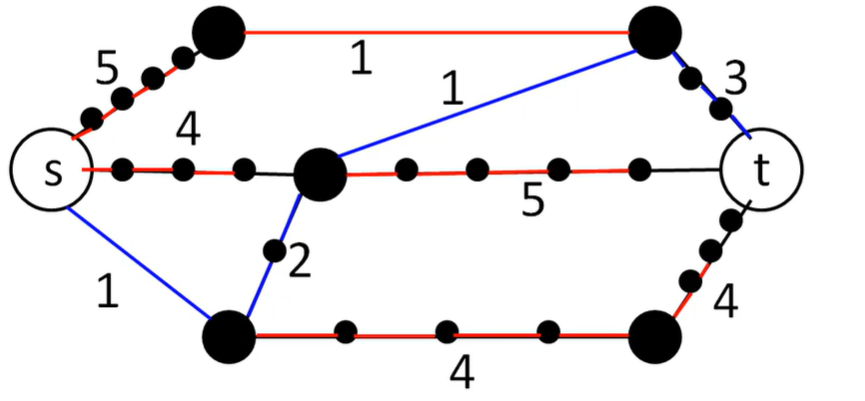
\includegraphics[scale=0.4]{../assets/bfs_unit_edges.png}
\end{center}
Here, we see that the blue path has distance 7 (the lowest) while the red paths are the other paths that the BFS algorithm took. 

\bigskip 

Now, this \emph{works}. However, there are some issues. 
\begin{itemize}
    \item BFS is linear time for the graph that we run it on. However, we're breaking this graph up so every edge can be represented as a unit edge (so an edge of weight $n$ becomes $n$ edges of weight 1). The runtime is $\BigO(\text{Sum of Edge Lengths})$.
    \item What if we have an edge of length one million? 
    \item What if our edges have decimal weights (e.g. $\pi$, $15.12314352452$, so on)?
\end{itemize}

\subsection{Another Way}
If we have very long edge lengths, most steps will just consist of advancing slightly (one unit) along a bunch of edges. The issue is, there may be a time period where all we're doing is advancing along one unit for each path that BFS is taking. 

\bigskip 

So, how do we ``fast forward'' through these boring steps? Well, occasionally, we have an interesting step where, for instance, the wavefront hits a new vertex. In other words, every time you hit a new vertex, you might need to update some things. But, ignoring that, all we're really doing is slowly advancing through each edge. 

\subsection{Algorithm}
This algorithm is associated with the ``ooze'' that was mentioned in lecture. 
\begin{verbatim}
    Distances(G, s, l)
        dist(v) = 0
        While not all distances found 
            Find minimum over (v, w) in E
                with v discovered w not 
                of dist(v) + l(v, w)
            dist(w) = dist(v) + l(v, w)
            prev(w) = v
\end{verbatim}

\subsubsection{Why Does This Work?}
\begin{proposition}
    Whenever the algorithm assigns a distance to a vertex $v$, that is the length of the shortest path from $s$ to $v$. 
\end{proposition}

\begin{mdframed}[]
    \begin{proof}
        We use induction.
        \begin{description}
            \item[Base Case:] We know that \code{dist(s) = 0}. The empty path has length 0. 
            \item[Inductive Step:] When assigning distances to $w$, suppose that all previously assigned distances are correct. We can imagine a bubble containing the vertices $s$ and $v$, with edge denoted by $\text{dist}(v)$. By the inductive hypothesis, we assume that all edge lengths inside this bubble is correct. Take a vertex $w$ which is outside of the bubble so that the path length from $v$ (inside the bubble) to $w$ has length $\ell(v, w)$. This is the shortest path from $s$ to any vertex outside the bubble. 
        \end{description}
    \end{proof}
\end{mdframed}

\subsubsection{Runtime of Initial Algorithm}
This runs in $\BigO(|V| \cdot |E|)$ time. There are $\BigO(|V|)$ iterations and $\BigO(|E|)$ edges.
\begin{itemize}
    \item This is too slow because every iteration we have to check every edge. 
    \item The idea is that most of the comparison doesn't change much iteration to iteration. So, we can use this to save time. 
    \item Specifically, record for each $w$ the best value of $\text{dist}(v) + \ell(v, w)$. 
\end{itemize}

\subsection{Better Algorithm}
Our better algorithm is based on the observations that we had above.
\begin{verbatim}
    Distances(G, s, l)
        For v in V 
            dist(v) = infinity 
            done(v) = false 
        dist(s) = 0
        done(s) = false 

        while not all vertices done 
            Find v not done with minimum dist(v)
            done(v) = true 
            For (v, w) in E 
                if dist(v) + l(v, w) < dist(w)
                    dist(w) = dist(v) + l(v, w)
                    prev(w) = v
\end{verbatim}
The initialization is $O(|V|)$, and the while loop is $\BigO(|V|)$. The for loop is $\BigO(|E|)$ time. Thus, the runtime is: 
\[\BigO(|V|^2 + |E|)\]
\begin{itemize}
    \item This repeatedly asks for the smallest vertex. Even though not much is changing from round to round, the algorithm is computing the minimum from scratch every time.
    \item We can use a data structure to help answer a bunch of similar questions faster than answering each question individually (like the one above).
\end{itemize}

\subsection{Priority Queue}
A \textbf{priority queue} is a data structure that stores elements sorted by a \textbf{key} value. Its operations are: 
\begin{itemize}
    \item \code{insert}: Adds a new element to the priority queue.
    \item \code{decreaseKey}: Changes the key of an element of the priority queue to a specified smaller value. 
    \item \code{deleteMin}: Deletes the element with the lowest key from the priority queue. 
\end{itemize}

\subsection{Even Better Priority Queue}
\begin{verbatim}
    Dijkstra(G, s, l)
        Initialize Priority Queue Q 
        For v in V
            dist(v) = infinity
            Q.insert(v) // using dist(v) as key
        dist(s) = 0
        while Q not empty
            v = Q.deleteMin()
            For (v, w) in E
                if dist(v) + l(v, w) < dist(w)
                    dist(w) = dist(v) + l(v, w)
                    prev(w) = v
                    // w has a faster path and needs to updated in
                    // the priority queue 
                    Q.decreaseKey(w)
\end{verbatim}
The runtime is as follows: 
\begin{itemize}
    \item We need to iterate $\BigO(|V|)$ times for the initial loop. 
    \item In the \code{while} loop, we run $\BigO(|V|)$ times. 
    \item We need to run through the edges $\BigO(|E|)$ times. 
\end{itemize}
So, $\BigO(|V|)$ \code{insert}s + $\BigO(|V|)$ \code{deleteMin}s + $\BigO(|E|)$ \code{decreaseKey}.

\end{document}